\documentclass{article}

% Remember to also load the algostyle.sty file into your project.
\usepackage{algostyle}

% Insert new packages here.

\begin{document}
\begin{question}
Let $A[1..n]$ be an array of $n$ distinct and positive integers. Given an integer $x$, describe an $O(n \log n)$ algorithm to return the number of distinct pairs $(i, j)$ of indices where $1 \leq i < j \leq n$, satisfying:
\begin{itemize}
    \item $A[i] > A[j]$, and
    \item $A[i] + A[j] = x$.
\end{itemize}

{\bfseries Note.} {\em This was an assignment problem from COMP3121/9101, 23T2.}
\end{question}

\begin{rubric}
\begin{itemize}
    \item This task will form part of the portfolio.
    \item Ensure that your argument is clear and keep reworking your solutions until your lab demonstrator is happy with your work.
\end{itemize}
\end{rubric}

\begin{solution}
    Perform a modified merge sort algorithm. 
    At each node in the recursion tree, after conquering but before merging, perform a modified two-sum algorithm on the two arrays to be merged.
    Start with a pointer $l$ to the leftmost element of the left subarray, and a pointer $r$ to the rightmost element of the right subarray.

\begin{center}


    \tikzset{every picture/.style={line width=0.75pt}} %set default line width to 0.75pt        

    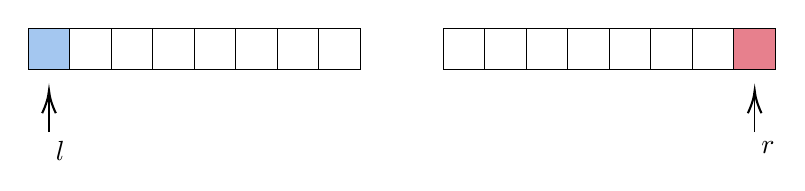
\begin{tikzpicture}[x=0.75pt,y=0.75pt,yscale=-1,xscale=1]
    %uncomment if require: \path (0,300); %set diagram left start at 0, and has height of 300
    
    %Shape: Grid [id:dp8843699222147772] 
    \draw  [draw opacity=0] (145.47,92) -- (305.47,92) -- (305.47,112) -- (145.47,112) -- cycle ; \draw   (165.47,92) -- (165.47,112)(185.47,92) -- (185.47,112)(205.47,92) -- (205.47,112)(225.47,92) -- (225.47,112)(245.47,92) -- (245.47,112)(265.47,92) -- (265.47,112)(285.47,92) -- (285.47,112) ; \draw    ; \draw   (145.47,92) -- (305.47,92) -- (305.47,112) -- (145.47,112) -- cycle ;
    %Shape: Grid [id:dp9924539760633466] 
    \draw  [draw opacity=0] (345.47,92) -- (505.47,92) -- (505.47,112) -- (345.47,112) -- cycle ; \draw   (365.47,92) -- (365.47,112)(385.47,92) -- (385.47,112)(405.47,92) -- (405.47,112)(425.47,92) -- (425.47,112)(445.47,92) -- (445.47,112)(465.47,92) -- (465.47,112)(485.47,92) -- (485.47,112) ; \draw    ; \draw   (345.47,92) -- (505.47,92) -- (505.47,112) -- (345.47,112) -- cycle ;
    %Straight Lines [id:da4140804502723001] 
    \draw    (155.47,142) -- (155.47,124) ;
    \draw [shift={(155.47,122)}, rotate = 90] [color={rgb, 255:red, 0; green, 0; blue, 0 }  ][line width=0.75]    (10.93,-3.29) .. controls (6.95,-1.4) and (3.31,-0.3) .. (0,0) .. controls (3.31,0.3) and (6.95,1.4) .. (10.93,3.29)   ;
    %Straight Lines [id:da28861266912498484] 
    \draw    (495.47,142) -- (495.47,124) ;
    \draw [shift={(495.47,122)}, rotate = 90] [color={rgb, 255:red, 0; green, 0; blue, 0 }  ][line width=0.75]    (10.93,-3.29) .. controls (6.95,-1.4) and (3.31,-0.3) .. (0,0) .. controls (3.31,0.3) and (6.95,1.4) .. (10.93,3.29)   ;
    %Shape: Rectangle [id:dp6086797401618855] 
    \draw  [fill={rgb, 255:red, 74; green, 144; blue, 226 }  ,fill opacity=0.5 ] (145.47,92) -- (165.47,92) -- (165.47,112) -- (145.47,112) -- cycle ;
    %Shape: Rectangle [id:dp4032157767240401] 
    \draw  [fill={rgb, 255:red, 208; green, 2; blue, 27 }  ,fill opacity=0.5 ] (485.47,92) -- (505.47,92) -- (505.47,112) -- (485.47,112) -- cycle ;
    
    % Text Node
    \draw (157.47,145.4) node [anchor=north west][inner sep=0.75pt]    {$l$};
    % Text Node
    \draw (497.47,145.4) node [anchor=north west][inner sep=0.75pt]    {$r$};
    
    
    \end{tikzpicture}
    
\end{center}

We will now begin a loop, where in each iteration, either the $l$ advances right, or $r$ advances left.
With every iteration, compare the sum of the elements $A[l]+A[r]$ with the target sum $x$.
If the sum is greater than $x$, then advance the $r$ pointer left. If the sum is less than $x$, then advance the $l$ pointer right.
If the sum is equal to $x$, then check if $A[l]>A[r]$. If this final condition is true, then increment the counter.
Terminate the loop when either pointer steps out of their own subarray.

\end{solution}
\end{document}